% #############################################################################
% This is Chapter 3
% !TEX root = ../main.tex
% #############################################################################
% Change the Name of the Chapter i the following line
\fancychapter{Problem Definition}
\cleardoublepage
% The following line allows to ref this chapter
\label{chap:problem}

This chapter will define the problem, the client requirements and list the necessary functionalities of the solution, to successfully address the problem.
First some context surrounding the problem is given. 
Next, the profile of the target clients will be described, and some examples will be given.
The following section contains a list of client requirements the solution must abide by.
Then it will shed the light on some essential concepts in order to understand the operations that need to be implemented.
It will end by detailing the client use cases it must provide.

% -----------------------------------------------------
% -----------------------------------------------------
\section{Context}\label{chap:problem:context}
As discussed before, the same computers commonly used for communications and information storage are exploitable by attackers, and can cause a minor inconveniences, to possibly severe repercussions, such as, losing your confidential data to malicious parties.

An interesting approach to improve security is to add another layer of security to confidential data and communications through the addition of an device, independent of the user's personal computer. The device is responsible for the security of sensitive data and communications.

% An illustration of the system with multiple users can be seen in figure~\ref{fig:main-system}.

\subsection{Entities}\label{chap:problem:entities}

These type of devices are especially relevant to people high responsibility jobs, that handle very sensitive information, which have dire consequences if they are lost, corrupted or leaked.
Some examples are government officials who handle confidential information pertaining to a country, company executives, such as the CEO who have access to company secrets, diplomats who manage confidential treaties, and military officers who have access to information critical to a countries' security.

% Talk about groups and individuals
Additionally, not just individuals have interest in these systems, a device can be assigned to a group of people representing an entity. For example, in the armed forces, a device can be assigned to the navy, one to the infantry, and every other faction. Any ranked officer, or people with a certain level of authority, could use the entity device, to communicate with other people or entities, in behalf of the group.

\subsection{Devices}\label{chap:problem:devices}
% Devices
There are currently on the market some dedicated devices designed to secure communications and save private data.
These type of devices have physical tamper-resistant measures against attackers who wish to read the device's information. They also provide fail-safe mechanisms in case of an attack.
\ac{HSM} is a high grade device, with more computational power and larger storage capacity for the user's secrets.

Smart Cards, provide secure and portable tamper-resistant storage.
They have lower processing power, and smaller memory which only allows to store a small amount of data.
They have a low-cost, so can be produced in bulk and easily replaced. Only an RFID card reader is needed to read its information, and verify the owner's identity.
Because of these features, they are widely used in the retail, healthcare, communication and government industries.

% -----------------------------------------------------
% -----------------------------------------------------
\section{Requirements}\label{chap:problem:requirements}

To effectively address the presented problem, there are several high-level requirements the solution must adhere to:
\begin{itemize}
	\item Devices should be distributable to individuals or entities with one or more individuals;
	\item The system must allow communications between individuals representing themselves or an entity;
	\item The system must be responsible for securing all communications against any sort of attacks;
	\item The device should be independent from user's personal computers;
	\item Users should be able to create secure communications with available and new entities;
	% \item New secure connections should be created, if existing communications are suspected to be compromised;
	\item It should provide an easy-to-use interface by everyone, including non-technical people;
	\item It should have a relatively low cost, to allow distribution of several devices among multiple people;
	\item Only authorized individuals should be able to use the device.
\end{itemize}

These client requirements need to be translated into slightly more technical and tangible requirements a solution must follow.
% -----------------------------------------------------
In order to secure communications, the following services must be guaranteed: confidentiality, integrity and authentication.
With asymmetric keys the system can provide non-repudiation to documents or files, by means of qualified digital signatures.

% -----------------------------------------------------
The device must store all keys related to the entity who owns the device.
The device must support secure storage in order to store the user's sensitive information, such as the cryptographic keys.
These keys must never be exposed to the outside environment of the device to ensure the security of communications and independence of the system.
All cryptographic operations must also be performed inside the device.
Additionally, the device should have physical tamper-resistant measures and mechanisms in place, in case of an intrusion, such as, permanent erasure of all sensitive data. 
This means that even if an attacker is in possession of the physical device, it should be extremely difficult or even impossible to extract any information from it.
% The solution should follow the \ac{PKCS} \#11 standards, to strengthen its security requirements.
% -----------------------------------------------------
% This is where the widely established standard \ac{PKCS} \#11 is again relevant. It allows operations to be standardized across different devices, increasing the range of supported devices.
% By implementing the system in accordance with these guidelines, it will have a higher device interoperability.

% -----------------------------------------------------
The solution should work with a plethora of devices, which will increase the adoptability of the solution among clients.
The system should provide an application on the user's device, which will communicate with the physical device, and make the operation's available to the user through a simple interface for the regular non-tech savvy user.
Another related requirement is the usage of a common connection solution, e.g. \ac{USB} cable, to further increase the pool of supported devices.
In addition, the system should perform the operations in a reasonable time to minimize the user's wait, and improve the user experience.

% -----------------------------------------------------
% -----------------------------------------------------
\section{Use Case Scenarios}\label{chap:problem:scenarios}

This section will define and detail the use cases the solution must satisfy and provide to the user. The combination of the use cases satisfy the client requirements in Section~\ref{chap:problem:requirements}.
Figure~\ref{fig:main-system} will be used as an example and illustration for the different scenarios.

\begin{figure}[h!]
    \centering
    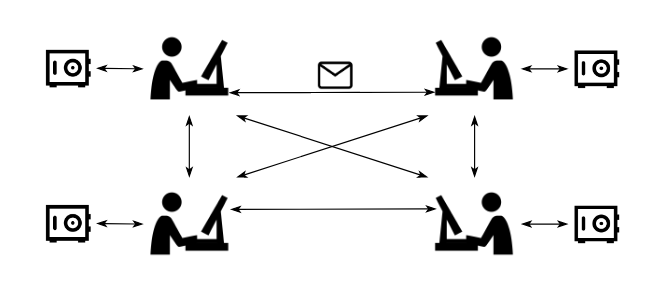
\includegraphics[width=0.7\textwidth]{./Images/main-figure.png}
    \caption{System Usage Example}
    \label{fig:main-system}
\end{figure}

% -----------------------------------------------------
\subsection{Authenticating the User}\label{chap:problem:scenarios:auth}

Every user must authenticate himself, before using the device. This can be done by providing a \ac{PIN}, which the device will verify before unlocking the session for the user.
The device will come from fabric with a default authentication \ac{PIN}. The users should be allowed to change this number.
For \textbf{personal} devices, there is only one user, the owner, as illustrated by Alice and Bob in figure~\ref{fig:main-system}. There is only the single authentication \ac{PIN}, which when sent to the device, unlocks the session, and the user can access its services.
For \textbf{groups} and entities, there can be multiple users, illustrated by Charlie. In this case, there are different scenarios for authentication.
The simplest is when it is not needed to authenticate the individual user, only the entity. There is only a single authentication \ac{PIN} for the entity. All the user's with permission to communicate in behalf of the entity, must know the \ac{PIN}. They only need to send the number to the device to be allowed access to its operations.

The second scenario, is when an entity wishes to authenticate each individual user with access to the device. 
This would entail a more complex process. A user will be assigned the role of administrator. For example, in the military, this could be assigned to the top ranking general. The administrator, using the administrator \ac{PIN}, is able to register new users with their own private \ac{PIN}, access the logs of which user logged in and when, as well as, which messages they sent and received.
The registration of a new user can be done physically with both administrator and user present. Afterwards, the registered user can use their credentials to authenticate himself, and use the entities device to communicate.
It is important to note that in all scenarios, only the users or the entity is authenticated, the device does not authenticate itself to the user.
% The administrator authenticates himself to the device, begins the registration process and allows the user to insert their name and \ac{PIN}.

% -----------------------------------------------------
\subsection{Secure Communications}\label{chap:problem:scenarios:comms}

%% SECURE COMMUNICATIONS %%
The main goal of the system is to enable secure communications. Communications can be setup between two or more entities. For each configured communication, the same symmetric key is saved in secure storage on each device. One key per communication.
For a user to send secure data, first he authenticates himself to the device, then sends the data to it. The device will return it secured. The user can then send it through a convenient offline service such as email, or an online chat service. Only a recipient with a similar device and the same key can read the data content.
% --------------------------

\begin{figure}[h!]
    \centering
    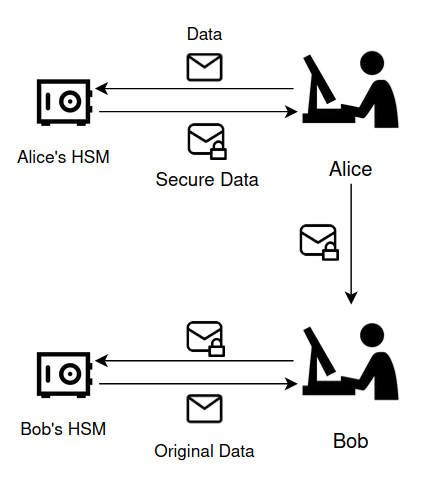
\includegraphics[width=0.5\textwidth]{./Images/user-data-service.png}
    \caption{Secure data exchange service example using internal keys}
    \label{fig:user:data-service}
\end{figure}

%% USAGE EXAMPLE %%
An possible usage example of secure data exchange between two users, Alice and Bob, is depicted in figure \ref{fig:user:data-service}. Firstly, Alice forwards the data, to be sent securely to Bob, to the device and the device returns the data secured with an internal key. Then, Alice can forward the result to any entity with the same internal key in their device, through a chat application, e-mail or other convenient service.
The receiver Bob sends the secure data to the device, and receives the original message.
This service should prevent any third party from gaining access to the data, or altering the message. The receiver can be confident of the data's origin. It could not have been sent by any malicious entity.

% These devices have a certain amount of secure storage, so there is a limit to the number of symmetric keys which can be stored there.
Each entity, upon ordering the device, should be able to specify which entities it wants to communicate with.
For example, Alice can request a device which enables two separate communication channels with Bob and Charlie, separately. Alice can also request a single channel with all three entities. In this case, only one key is required for all.
Before devices are delivered, the keys will be generated and stored in the necessary device. When all involved entities receive their device, they can begin secure communications immediately.

%% COMMUNICATION CHANNELS LIMIT %%
The device should not have a practical limit on the amount communication channels it can establish. This means it should have a reasonable amount of keys storage space
If the device's secure storage is limited, then a solution using symmetric or asymmetric keys to secure all other keys on regular, higher capacity non-volatile memory.
This gives entities the flexibility needed to communicate with the number of entities they wish.

%% QUALIFIED DIGITAL SIGNATURES %%
Another scenario includes a pair of asymmetric keys generated inside each device, and never exposed to the outside. This allows the generation of qualified \textbf{digital signatures}, which can legally represent the entity.
Then for example, when a user wishes to generate a signature for a piece of data, he must send the data to the device, which computes and returns the signature to the user.
% Each device has a pair of asymmetric keys stored in secure storage, generated inside the device from fabric. These keys allow the storage of a practically unlimited number of symmetric keys in non-volatile memory.
% This feature is useful in other situations. There are cases where existing symmetric keys might need to be revoked, due to suspicion of being compromised, with new ones generated and shared.
% Another case is if the symmetric key has an expiration date, when it expires, new keys need to be exchanged.

% Finally, when using asymmetric keys, beyond providing authentication to the communications, the data sender can be authenticated to the receiver, using the entities private key stored in the device.

% -----------------------------------------------------
\subsection{New Communications}\label{chap:problem:scenarios:keys}

%% REASONING FOR SERVICE %%
The operations described so far provide a usable and functional system to organizations and users, but it is not very flexible. It does not allow users to communicate with new entities without returning the device to manufacturing to be equipped with the necessary information.
To avoid this, a service should be available to users with usable devices in their possession, to trade data with another entity with an identical device, which the device could not previously. It should be easy to provide the functionality without burdening the user with more responsibility or complex tasks.

%% SERVICE PRESENTATION %%
A possible solution is the inclusion of a control station, where the user's originally collect their devices. Each device is delivered with its own communication channel with the control station. Effectively this station is treated as another entity.
Whenever users wish to communicate with another user, they can send a list of the entities the user intents to communicate, secured with the data exchange service. The control station subsequently supplies the user with the necessary information to be imported in their device.

\begin{figure}[h]
    \centering
    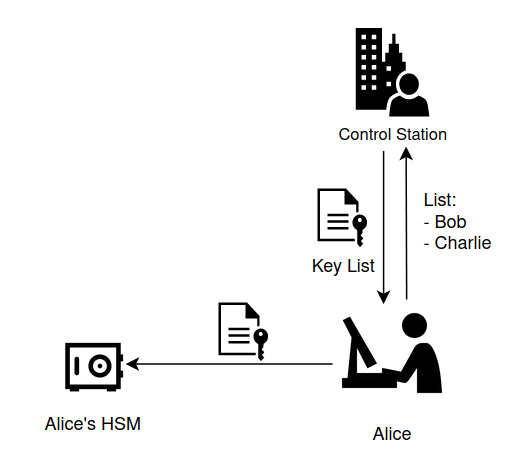
\includegraphics[width=0.65\textwidth]{./Images/user-import-service.png}
    \caption{Import key list to device usage example}
    \label{fig:user:import-service}
\end{figure}

%% USAGE EXAMPLE %%
A use case scenario of this service is depicted in figure \ref{fig:user:import-service}.
Alice forwards the list with the names of entities to the control station, which returns the key list to Alice. The list can be forwarded to the device, and the new keys are stored and immediately ready for use with Bob and Charlie, as soon they import their list in their devices. 
Users can then resume communications, using the secure data exchange service, with minimal interruption.

%% ADVANTAGES / POSSIBILITIES %%
The service offers the possibility of setting up a regular communication update schedule. It grants the flexibility of key revocation when needed, data exchange with new entities, as well as updating communication keys which have reached their expiration date, with no additional complexity to the user, to always safeguard the security of communications.
Expiration dates on keys adds longevity to the system. It avoids overuse, and reduces the possibility of compromised connections. When keys expire, new ones can be delivered.
Another, less cumbersome possibility for the user, is whenever an entity is added to system and receives a device, the station delivers a message to each entity with the updated key list. The list can be imported by each user if needed.

% The list can be sent using an offline service such as email. Every time a new entity is added to the list, the station sends a new email with the updated list. Each entity can get access these updates when they need it.

% Each month an entity can hand over a list of the entities it wishes to communicate with to the control station, which will accordingly yield the corresponding key set, as pictured in figure \ref{fig:user:import-service}.
% Each entity only needs to forwards the list to the device, and the new keys are immediately stored and ready to be used.


% The list can be provided at the manufacturing control station, when the device is delivered.
% Afterwards, there are two options to distribute the list. When the list is updated with new entities, a member of the entity will physically go to the station, to retrieve it.
% Alternatively, the entity will receive the device with the necessary keys to securely communicate with the control station. When an entity needs the list, it will be supplied for them by the control station. In this scenario, the control station can be thought of as a special entity.

% Adding to the previous scenario with asymmetric keys, users will be able to establish secure communications with new entities. This is achieved by distributing a list of available entities to communicate with.
% When and individual, e.g. Alice, wants to establish communications with a new entity, such as Bob, she needs to get Bob's key from the received list. Then they can securely trade a new key, and begin communications.
